\section{Theoretical Analysis}
\label{sec:analysis}

\par In this section, the explanation of the theoretical analysis of the circuit showed in the introduction is given. For this analysis the ideal model for the OP-AMP was used, in which $Z_{in}$ is infinite and $Z_{out}$ is zero.

\par First, the lower and upper cut-off frequencies were computed. These calculations using Octave were based on:

\begin{equation}
  \omega_{L} = \frac {1}{R1*C1}.
  \label{eq:eq1}
\end{equation}

\begin{equation}
  \omega_{H} = \frac {1}{R2*C2}.
  \label{eq:eq2}
\end{equation}

\par Consequently, the central frequency was determined using the following expression:

\begin{equation}
  \omega_{C} = \sqrt{\omega_{L}*\omega_{H}}.
  \label{eq:eq3}
\end{equation}

\par The next step was to determine the transfer fuction of the circuit, in order to compute the frequency response of the gain and also to get the gain at the central frequency as requested. An analysis of the circuit culminated in the following expression for this function:

\begin{equation}
  T(s) = \frac{V_{out}(s)}{V_{in}(s)} = \frac{R1*C1*s}{1 + (R1*C1*s)}*(1+\frac{R3 + R5}{R4})*\frac{1}{1 + (R2*C2*s)}.
  \label{eq:eq3}
\end{equation}

\par With $s=j*w$.

\par Using this expression and substituting $s$ by $j*\omega_{C}$, the gain at the central frequency was determined. With these results, Table\ref{tab:tr1} was produced:

\begin{table}[h]
  \centering
  \begin{tabular}{|l|r|}
    \hline    
    {\bf Name} & {\bf Value}\\ \hline
    $Lower Cut-off Frequency [Hz]$ & 7.234316e+02 \\ \hline 
$Upper Cut-off Frequency [Hz]$ & 1.446863e+03 \\ \hline 
$Central Frequency [Hz]$ & 1.023087e+03 \\ \hline 
$Gain [dB]$ & 4.254210e+01 \\ \hline 

  \end{tabular}
  \caption{Frequency and gain.}
  \label{tab:tr1}
\end{table}

\par Using the transfer function, a frequency analysis was made. With this, we were able to produced two graphics that show the frequency response of both the gain(dB) and phase(degrees). Figures \ref{fig:gain} and \ref{fig:phase} show exactly this:

\begin{figure}[h] \centering
\includegraphics[width=0.6\linewidth]{gain.eps}
\caption{Frequency response - Gain(dB) .}
\label{fig:gain}
\end{figure}

\newpage

\begin{figure}[h] \centering
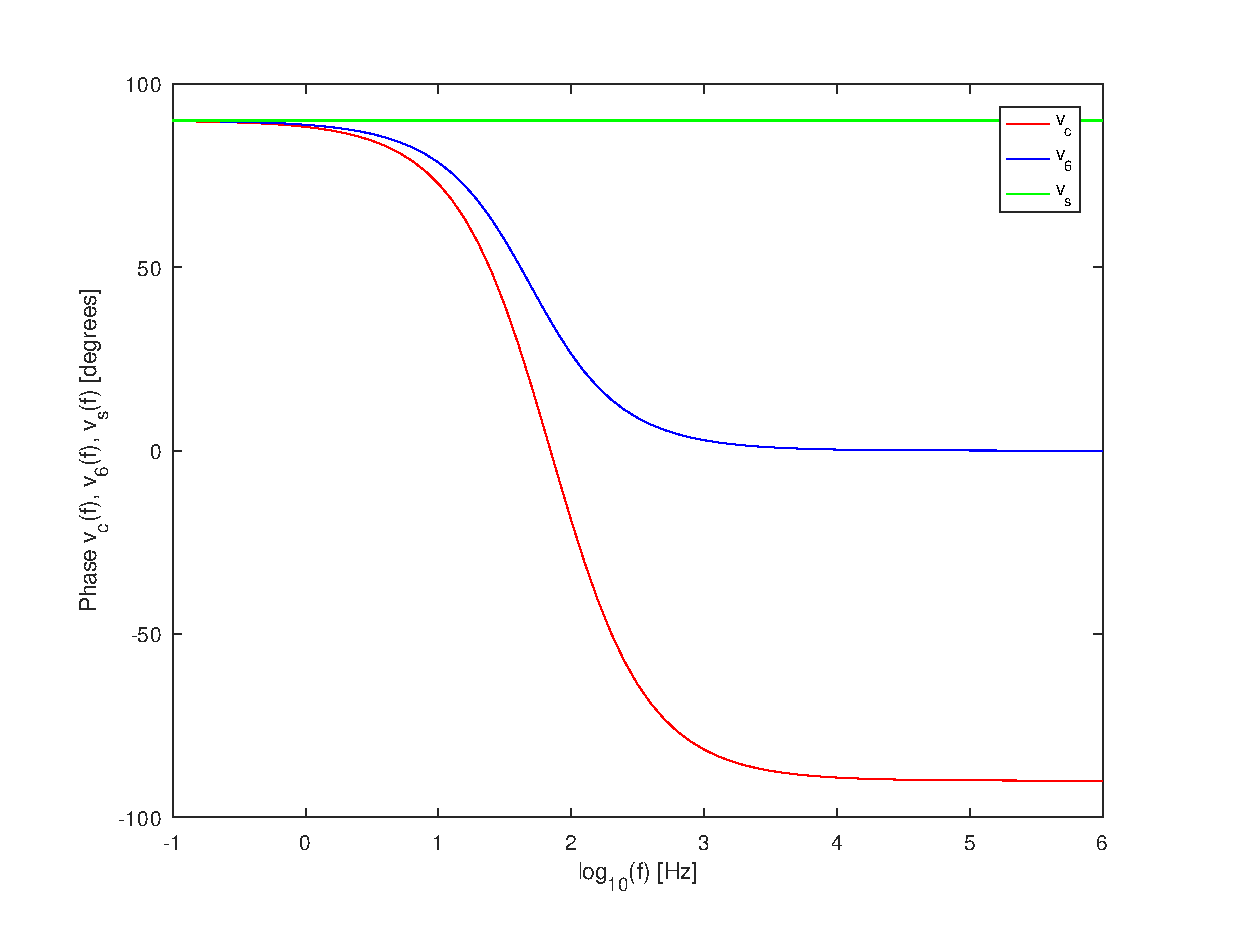
\includegraphics[width=0.6\linewidth]{phase.eps}
\caption{Frequency response - Phase(degrees) .}
\label{fig:phase}
\end{figure}


\par After this frequency analysis, the input and output impedances were computed using the value for the central frequency previously calculated. These impedances were obtained using the expressions below:

\begin{equation}
  Z_{in} = R1 +  \frac{1}{j*\omega_{C}*C1}.
  \label{eq:eq4}
\end{equation}

\begin{equation}
  Z_{out} = \frac{1}{\frac{1}{R2} + j*\omega_{C}*C2}.
  \label{eq:eq5}
\end{equation}

\par With these calculations, the obtained results for the theoretical impedances were:

\begin{table}[h]
  \centering
  \begin{tabular}{|l|r|}
    \hline    
    {\bf Name} & {\bf Value}\\ \hline
    $Input impedance$ & 1.224745e+03 \\ \hline 
$Output impedance$ & 8.164966e+02 \\ \hline 

  \end{tabular}
  \caption{Input and output impedances at central frequency.}
  \label{tab:tr2}
\end{table}

\newpage

\par Finally, the gain and frequency deviations were computed (comparing to the values of 40dB for the gain and 1kHz for the central frequency) and also the cost and merit. With this, Table\ref{tab:tr3} was produced in order to evaluate the circuit in terms of its efficiency:

\begin{table}[h]
  \centering
  \begin{tabular}{|l|r|}
    \hline    
    {\bf Name} & {\bf Value}\\ \hline
    $Gain Deviation [V]$ & 1.340000e+00 \\ \hline 
$Central Frequency Deviation [Hz]$ & 2.308672e+01 \\ \hline 
$Cost$ & 1.352633e+04 \\ \hline 
$Merit$ & 3.026597e-06 \\ \hline 

  \end{tabular}
  \caption{Merit calculations.}
  \label{tab:tr3}
\end{table}

\newpage
